\documentclass[11pt]{article}
\renewcommand*\rmdefault{ppl}
\usepackage{authblk}
\usepackage[letterpaper, margin=1.2in]{geometry}
\usepackage{hyperref}
\usepackage[superscript,biblabel]{cite}
\usepackage{ragged2e}
\usepackage{caption}
\usepackage{graphicx}
\bibliographystyle{unsrt}

\title{DOTA2 Match Result Prediction Based On Hero Lineups}
\author[1]{Team 509\\Zhaoyin Zhu}
\author[2]{Shuang Zhou}
\affil[1]{Division of Biostatistics, School of Medicine, New York University}
\affil[2]{Department of Computer Science, New York University}

\begin{document}
\maketitle

\section{Introduction}
Dota 2 is a free-to-play multiplayer online battle arena (MOBA) video game developed and published by Valve Corporation. The game was released for Microsoft Windows, OS X, and Linux in July 2013, following a Windows-only public beta testing phase that began in 2011, and is the stand-alone sequel to Defense of the Ancients (DotA), a modification for Warcraft III: Reign of Chaos and its expansion pack, The Frozen Throne \cite{dota2}.\\

\noindent Dota 2 is played in matches between two five-player teams, represented by the name ``dire" and ``radiant", each of which occupies a stronghold in a corner of the playing field. A team wins by destroying the other side's "Ancient" building, located within the opposing stronghold. Each player controls one of 113 playable "Hero" characters that feature unique powers and styles of play. During a match, the player collects gold, items, and experience points for their Hero, while combating Heroes of the opposite team \cite{dota2}.

\section{Motivation}
ESports are getting growing attention and popularity. An increasing number of tournaments are being held, among which one of the most followed is ``The International" (TI). In 2015, the fifth TI tounament (TI5) in Seattle had the largest prize pool in eSports history, with a total of \$10.9 million\cite{ti5}. Therefore, it is very worthwhile to research the strategies and tactics within the game to have a better chance against competitions,yet this is a very new ground awaiting discovery. This is the motivation of our project: we want to propose a programmatic stratedy to pick out a lineup that puts a team in the driver seat before the match even begins.\\

\noindent Each match in Dota starts with the players picking their heroes. This stage of a match is much more important than it seems, and very often a bad lineup will pretty much rule the team out. In this stage, two teams take turns to ban and pick heroes, one at a time, until all 10 players have their corresponding heroes. A lot of strategies can be applied during the banning and picking. To name a few, a team may want to ban the heroes that worked really well for the opposing team before, or they want to counter a specific hero in the opposing lineup by picking one that can contain it with a later pick, or they want to achieve a $1+1>2$ effect by designing their lineup in a way that heroes supplement each other. Our project is to materialize those strategies and come up with an ideal lineup.

\section{Data}
The raw data we have is two database tables with very detailed descriptions of 12000 matches. We will only describe the revelant fields in the scope of this project. Table \ref{matches} shows the summary for database table MATCHES, and table \ref{players} shows the summary for database table PLAYERS. The two tables will be joined to form one single table that contains all heroes picked within the matches.

\begin{table}[h]
  \begin{center}
	\begin{tabular}{| c | c | c |}\hline
		field & type & description \\\hline
		match\_id & String & identifier for a match \\\hline
		radiant\_win & String & 0 if dire win, 1 if radiant win \\\hline
		human\_players & Integer & number of human players \\\hline
	\end{tabular}
	\caption{Summary for table: MATCHES}\label{matches}
  \end{center}
\end{table}

\begin{table}[h]
	\begin{center}
		\begin{tabular}{| c | c | c |}\hline
			field & type & description \\\hline
			match\_id & String & identifier for a match \\\hline
			hero\_id & String & identifier for each hero \\\hline
			win & Integer & 0 if the player lose, 1 if win \\\hline
		\end{tabular}
		\caption{Summary for table: PLAYERS}\label{players}
	\end{center}
\end{table}

\section{Objective}
We have established two capstones for this project. The first capstone and the primary objective is to predict the outcome of a match given only the lineups. Of course this prediction is made under the assumption that both sides perform around the same level. After the first capstone, we will try to generate a sequence of picks in response to another sequence of picks to simulate the actual hero selection stage.

\subsection{Match Outcome Prediction}
The objective here is to make a binary prediction indicating whether ``radiant" side can win based on the lineups of two sides.

\subsection{Pick Sequence Generation}
In the hero selection stage, two sides take turn to pick heroes, one at a time. So the objective here is to recommend picks given two partial, possibly empty, lineups. Each recommendation made will take into account the changes of lineups since last recommendation.

\section{Methods}
In order to achieve desirable prediction accuracy, we will include 3 types of features as potential predictors: single heroes ($p_1$ = 226), joint combinations of two heroes on the same side ($p_2$ = 12656), joint combinations of two heroes on the opposite side ($p_3$ = 12656). All the features are 0/1 variables and with these 3 types of features, we are able to account for both synergistic effect and antagonistic effect.\\ 

\noindent In our dataset, we only have 12000 matches (n = 12000), and the total number candidate predictors $p = p_1 + p_2 + p_3 = 25538$. In this case, we may encounter some difficulties since dimension $p$ is larger than sample size $n$. The design matrix $X$ is rectangular, having more columns than rows and the matrix $X^TX$ is huge and singular. The maximum spurious correlation between a covariate and the response can be large because of the dimensionality and the fact that an unimportant predictor can be highly correlated with the response variable due to the presence of important predictors associated with the predictor. To reduce dimensions and remove unnecessary predictors on ultrahigh dimensional data, sure independence screen (SIS) which is based on the correlation between predictors and outcome \cite{SIS} will be used to reduce $p$ close to $n$. After that, standard variable selection methods like Lasso\cite{lasso} and adaptive Lasso\cite{adalasso} will be utilized to fit the final model. \\

\noindent In modeling our data, we will try both nonparametric methods (decision tree, random forest) and parametric methods (SVM, logistic regression). In order to evaluate the performance of different methods, the dataset will be randomly split into training set ($n_{training} = 10000$) and testing set ($n_{test} = 2000$). Sensitivity and specificity will be reported to assess the accuracy of our model, and running time will be presented as well. 

\section{Results}
\subsection{Predicting Match Results}
\subsubsection{Feature Selection as part of the Model}
The number of features in this case is slight larger than the number of instances we have, thus for linear model such as Logistic Regression to work, we need to do a feature selection. The traditional way is to decide what features are useful and disregard all others in the model. However, online games like DOTA2 has some characteristics that may render the traditional feature selection inappropriate:
\begin{enumerate}
\item New heroes are constantly added as the game evolves.
\item New patches are coming out all the time.
\item There are always new trendings of tactics and strategies.
\end{enumerate}

\noindent These may caused some issues when the old features remained in the model appear less frequently and new important features that come about are ignored regardless. Then the model will suffer from performance loss unless rebuilt entirely.\\
\\
A more provident way is to let the model adapt to new features and select them with some certain cretiria. That is, we are buiding into the model a feature selection precess, instead of giving it a bunch of features we have already picked out.\\
\\
After some trials, we find out that cutting off features by their number of appearances in the dataset has random effect on performance, that is, no obvious relation between the threshold we set and the accuracy we obtain is observed. Thus we decide to go with selection by computing Pearson product-moment correlation coefficients.

\begin{center}
\captionof{table}{Feature Selection By Logistic Regression}
\begin{tabular}{| c | c | c | c |}\hline
Count Cut-off & Correlation Cut-off & Training Accuracy & Test Accuracy \\\hline
	10 & 0.015 & 0.7338 & 0.6715 \\\hline
	10 & 0.02 & 0.6863 & 0.6595 \\\hline
	20 & 0.01 & 0.7780 & 0.6665 \\\hline
	20 & 0.015 & 0.7284 & 0.6650 \\\hline
	20 & 0.02 & 0.6795 & 0.6510 \\\hline
\end{tabular}
\end{center}
A figure is given before to summarize the results.
\begin{center}
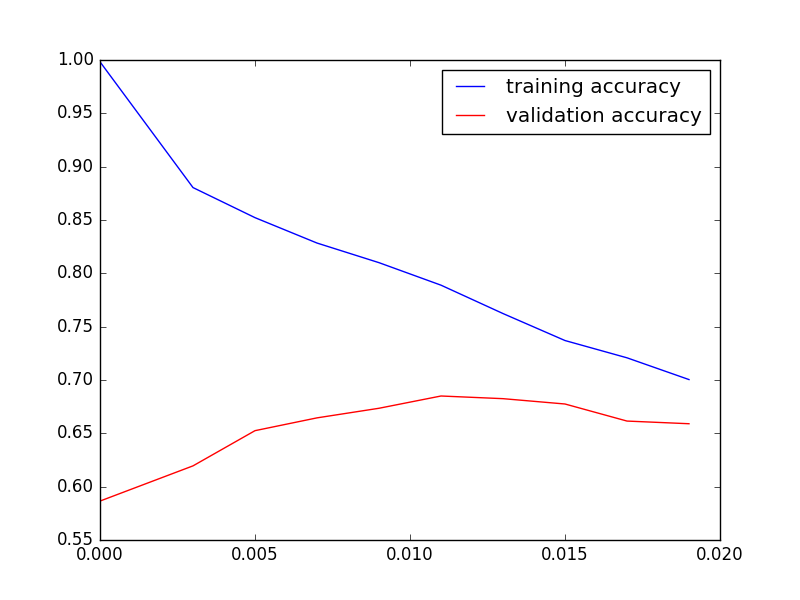
\includegraphics[scale=0.6]{big_interval.png}
\captionof{figure}{Accuracy With Different Correlation Cut-off}
\end{center}
When we cut off features with a correlation lower than 0.011, the model gives the highest validation accuracy. Therefore, we will go along with 0.011 as the correlation threshold with any future dataset.

\begin{thebibliography}{9}
	\bibitem{dota2} \url{https://en.wikipedia.org/wiki/Dota_2}, Wikipedia, accessed at March 21, 2016.
	\bibitem{ti5} \url{https://en.wikipedia.org/wiki/The_International_2015}, Wikipedia, accessed at March 21, 2016.
	\bibitem{SIS} Fan, J., \& Lv, J. (2008). Sure independence screening for ultrahigh dimensional feature space. \emph{Journal of the Royal Statistical Society: Series B (Statistical Methodology)}, 70(5), 849-911.
	\bibitem{lasso} Tibshirani, R. (1996). Regression shrinkage and selection via the lasso. \emph{Journal of the Royal Statistical Society. Series B (Methodological)}, 267-288.
	\bibitem{adalasso} Zou, H. (2006). The adaptive lasso and its oracle properties. \emph{Journal of the American statistical association}, 101(476), 1418-1429.
\end{thebibliography}
\end{document}
